%!TEX root = main.tex
\clearpage
\section{Conclusion}

\subsection{Global Vision}

In table \ref{tab:operators_status}, it's possible to understand the operators that was implemented in the first semestre of this dissertation. As can be seen, I have implemented \red{five} of thirteen operators that João Durães was especified.


\begin{table}[ht]
\begin{tabular}{c}
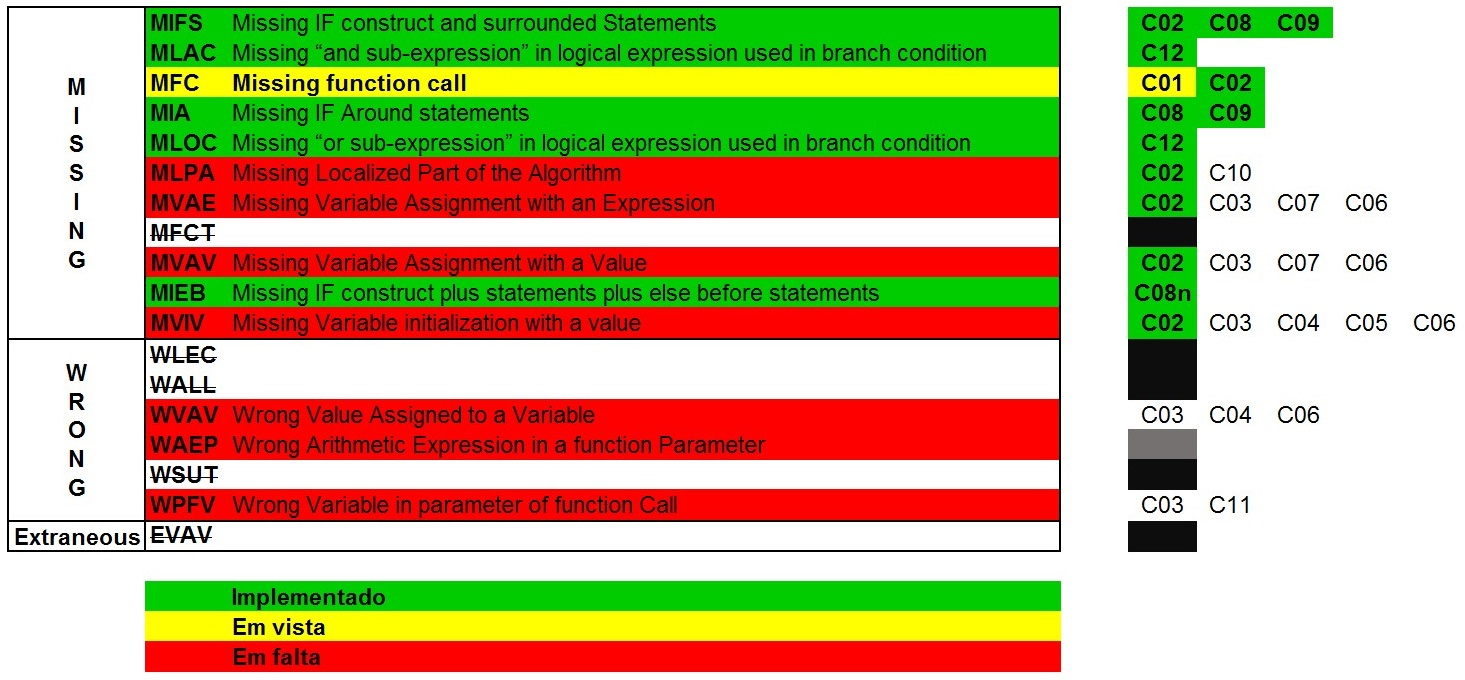
\includegraphics[width=1.1\textwidth]{img/operators_status.jpg}
\end{tabular}
\caption{\small \sl Operators Status and related constraints.\label{tab:operators_status}}
\end{table}


In table \ref{tab:constraints_status}, can be seen also that I have implemented \red{tree} of eleven constraints related to the thirteen operators.

\begin{table}[ht]
\begin{tabular}{c}
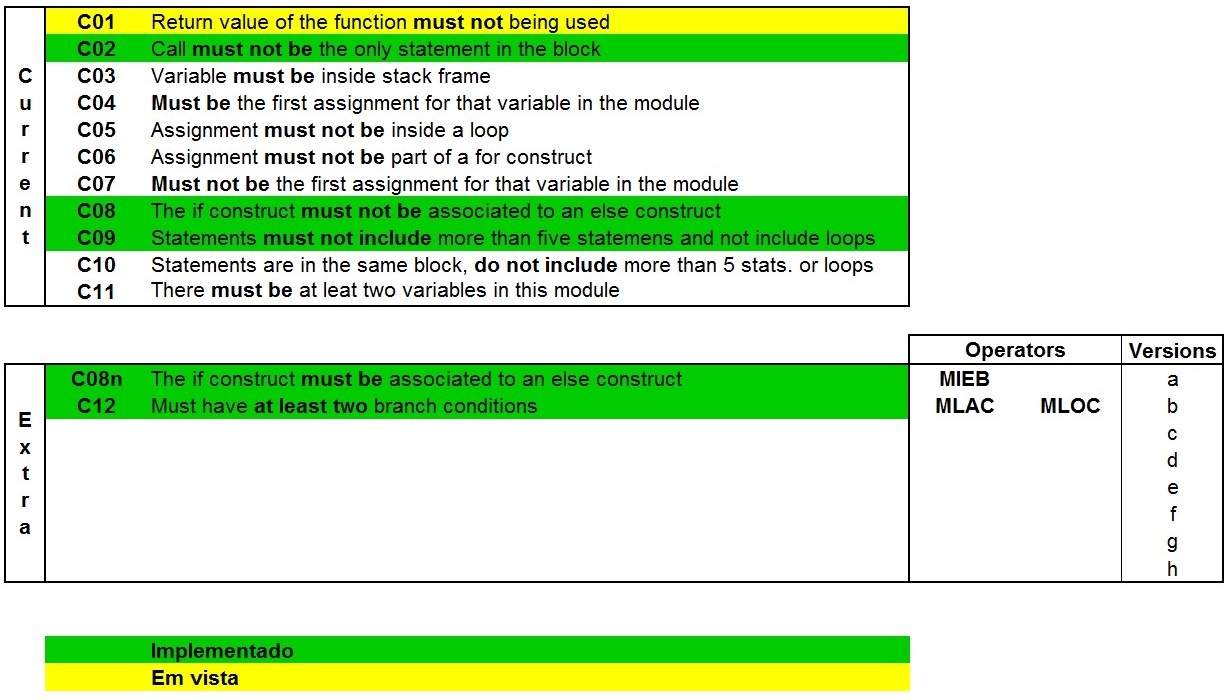
\includegraphics[width=1.1\textwidth]{img/constraints_status.jpg}
\end{tabular}
\caption{\small \sl Constraints Status.\label{tab:constraints_status}}
\end{table}

\clearpage
\subsection{Future Work}

To the future, I plain to implement the other operators and constraints. And apply this software in testing of open source softwares that I will select.